\subsubsection{Swarm EFI LP and FP data products}

\begin{verbatim}
import datetime
import matplotlib.pyplot as plt
import numpy as np
import pathlib

import geospacelab.visualization.mpl.dashboards as dashboards
\end{verbatim}

\paragraph{Swarm EFI LP 1B data}

\begin{verbatim}
def test_swarm_EFI_LP_1B_overview():
    """Test Swarm EFI/LP 1B data product
    
    """
    dt_fr = datetime.datetime(2016, 3, 14, 20, 15)
    dt_to = datetime.datetime(2016, 3, 14, 21, 0)

    db = dashboards.TSDashboard(
        dt_fr=dt_fr, dt_to=dt_to, figure_config={'figsize': (8, 10)},
        timeline_extra_labels=['GEO_LAT', 'GEO_LON', 'APEX_LAT', 'APEX_LON', 'APEX_MLT'],
        )

    ds = db.dock(
        datasource_contents=['esa_eo', 'swarm', 'l1b', 'efi_lp'], 
        product_version='latest', # 'latest' (default),
        sat_id='A', add_APEX=True)
    ds.list_all_variables()
    
    panel_layouts = [
        [ds['n_i'], ds['n_e']],
        [ds['T_e']],
        [ds['V_SC']],
        [ds['FLAG_LP'], ds['FLAG_n_i'], ds['FLAG_n_e'], ds['FLAG_T_e'], ds['FLAG_V_SC']],
        [ds['FLAG_1_BIN_AUX'],],
        [ds['FLAG_2_BIN_AUX'],],
    ]
    # Change some default attrs for better visualization
    ds['T_e'].visual.axis[1].lim = [ -10, 10000]

    db.set_layout(panel_layouts=panel_layouts)
    db.draw()
    db.add_title(title='Swarm -{} EFI/LP 1B Overview'.format(ds.sat_id), fontsize='medium', append_time=True)

    db.show()
test_swarm_EFI_LP_1B_overview()
\end{verbatim}

\begin{verbatim}
Create a new figure: Figure(800x1000).
Searching the data product "EFI_LP" with the version "latest" on the server...
INFO: Indexing the files for the product EFI_LP of the satellite A ...
The file [PosixPath('/data/afys -ionosphere/data/ESA/SWARM/Level1b/EFI_LP/0701/Sat_A/2016/SW_OPER_EFIA_LP_1B_20160314T000000_20160314T235959_0701_MDR_EFI_LP.cdf')] already exists: skip downloading.
/opt/anaconda3/envs/Swarm/lib/python3.12/site -packages/numpy/_core/numeric.py:442: RuntimeWarning: invalid value encountered in cast
  multiarray.copyto(res, fill_value, casting='unsafe')
Dataset: esa/earthonline | swarm | efi | efi_lp
Printing all of the variables ...
|No.                 |Variable name                 |Variable name (Source)        |Description                                                                                         |
| - - - - - - - - - - - - - - - - - - - -| - - - - - - - - - - - - - - - - - - - - - - - - - - - - - -| - - - - - - - - - - - - - - - - - - - - - - - - - - - - - -| - - - - - - - - - - - - - - - - - - - - - - - - - - - - - - - - - - - - - - - - - - - - - - - - - - - - - - - - - - - - - - - - - - - - - - - - - - - - - - - - - - - - - - - - - - - - - - - - - - - -|
|1                   |SC_DATETIME                   |N/A                           |Time of observation                                                                                 |
|2                   |Sync_Status                   |SyncStatus                    |                                                                                                    |
|3                   |SC_GEO_LAT                    |Latitude                      |Geographic Latitude                                                                                 |
|4                   |SC_GEO_LON                    |Longitude                     |Geographic Longitude                                                                                |
|5                   |SC_GEO_r                      |N/A                           |                                                                                                    |
|6                   |v_SC_ITRF                     |U_orbit                       |S/C velocity in ITRF                                                                                |
|7                   |n_i                           |N_ion                         |Ion density                                                                                         |
|8                   |CALIB_n_i                     |dN_ion                        |Calibration parameter for n_i, wrt. ISRs                                                            |
|9                   |n_i_err                       |N_ion_error                   |                                                                                                    |
|10                  |n_e                           |N_elec                        |Electron density                                                                                    |
|11                  |n_e_err                       |N_elec_error                  |                                                                                                    |
|12                  |T_e                           |T_elec                        |Electron temperature                                                                                |
|13                  |T_e_err                       |T_elec_error                  |                                                                                                    |
|14                  |CALIB_T_e                     |dT_elec                       |Calibration parameter for T_e, wrt. ISRs                                                            |
|15                  |V_SC                          |Vs                            |S/C potential                                                                                       |
|16                  |V_SC_err                      |Vs_error                      |                                                                                                    |
|17                  |FLAG_LP                       |Flags_LP                      |Flag of source: 1, 5, 9                                                                             |
|18                  |FLAG_n_i                      |Flags_N_ion                   |Flag of n_i: 10 - 40                                                                                |
|19                  |FLAG_n_e                      |Flags_N_elec                  |Flag of n_e: 10 - 40                                                                                |
|20                  |FLAG_T_e                      |Flags_T_elec                  |Flag of T_e: 10 - 40                                                                                |
|21                  |FLAG_V_SC                     |Flags_Vs                      |Flag of V_SC: 20, 30                                                                                |
|22                  |FLAG_BITS_1                   |Flagbits1                     |Binary flag (Instrument)                                                                            |
|23                  |FLAG_BITS_2                   |Flagbits2                     |Binary flag (Gain)                                                                                  |
|24                  |FLAG_1_BIN_AUX                |N/A                           |Binary flag (Instrument)                                                                            |
|25                  |FLAG_2_BIN_AUX                |N/A                           |Binary flag (Gain)                                                                                  |
|26                  |FLAG_1_BIN_IND                |N/A                           |                                                                                                    |
|27                  |FLAG_2_BIN_IND                |N/A                           |                                                                                                    |
|28                  |Gamma_1                       |Gamma1                        |                                                                                                    |
|29                  |Gamma_2                       |Gamma2                        |                                                                                                    |
|30                  |SC_APEX_LAT                   |N/A                           |APEX Latitude                                                                                       |
|31                  |SC_APEX_LON                   |N/A                           |APEX Longitude                                                                                      |
|32                  |SC_APEX_MLT                   |N/A                           |APEX Magnetic Local Time                                                                            |
|33                  |SC_GEO_LST                    |N/A                           |Local Solar Time                                                                                    |
\end{verbatim}

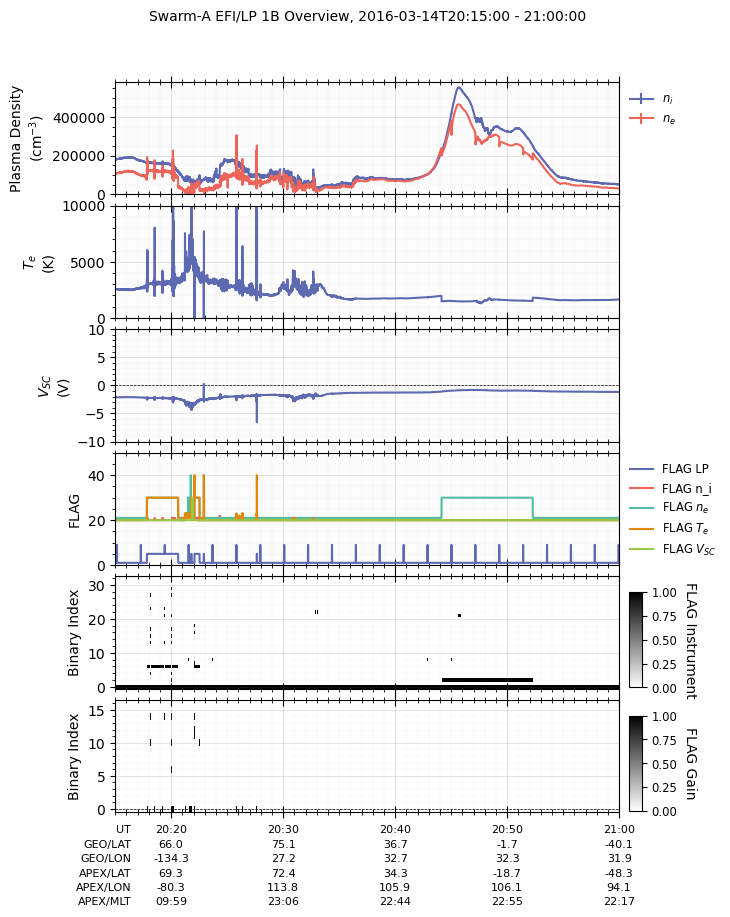
\includegraphics[width=0.7\linewidth]{files/0d82b0913aa228e966802f5e183f1ad5.png}

\paragraph{Swarm EFI LPI data}

\begin{verbatim}
def test_swarm_EFI_LPI_1B_overview():
    """Test Swarm EFI/LPI 1B data product
    
    """
    dt_fr = datetime.datetime(2016, 3, 14, 20, 15)
    dt_to = datetime.datetime(2016, 3, 14, 21, 0)

    db = dashboards.TSDashboard(
        dt_fr=dt_fr, dt_to=dt_to, figure_config={'figsize': (8, 10)},
        timeline_extra_labels=['GEO_LAT', 'GEO_LON', 'APEX_LAT', 'APEX_LON', 'APEX_MLT'],
        )

    ds = db.dock(
        datasource_contents=['esa_eo', 'swarm', 'l1b', 'efi_lpi'], 
        product_version='latest', # 'latest' (default),
        sat_id='A', add_APEX=True)
    
    panel_layouts = [
        [ds['n_i'], ds['n_e']],
        [ds['T_e']],
        [ds['V_SC']],
        [ds['FLAG_LP'], ds['FLAG_n_i'], ds['FLAG_n_e'], ds['FLAG_T_e'], ds['FLAG_V_SC']],
        [ds['FLAG_1_BIN_AUX'],],
        [ds['FLAG_2_BIN_AUX'],],
    ]
    # Change some default attrs for better visualization
    ds['T_e'].visual.axis[1].lim = [ -10, 10000]

    db.set_layout(panel_layouts=panel_layouts)
    db.draw()
    db.add_title(title='Swarm -{} EFI/LPI 1B Overview'.format(ds.sat_id), fontsize='medium', append_time=True)

    db.show()
test_swarm_EFI_LPI_1B_overview()
\end{verbatim}

\begin{verbatim}
Create a new figure: Figure(800x1000).
Searching the data product "EFI_LPI" with the version "latest" on the server...
The file [PosixPath('/data/afys -ionosphere/data/ESA/SWARM/Level1b/EFI_LPI/0701/Sat_A/2016/SW_OPER_EFIALPI_1B_20160314T000000_20160314T235959_0701_MDR_EFILPI.cdf')] already exists: skip downloading.
\end{verbatim}

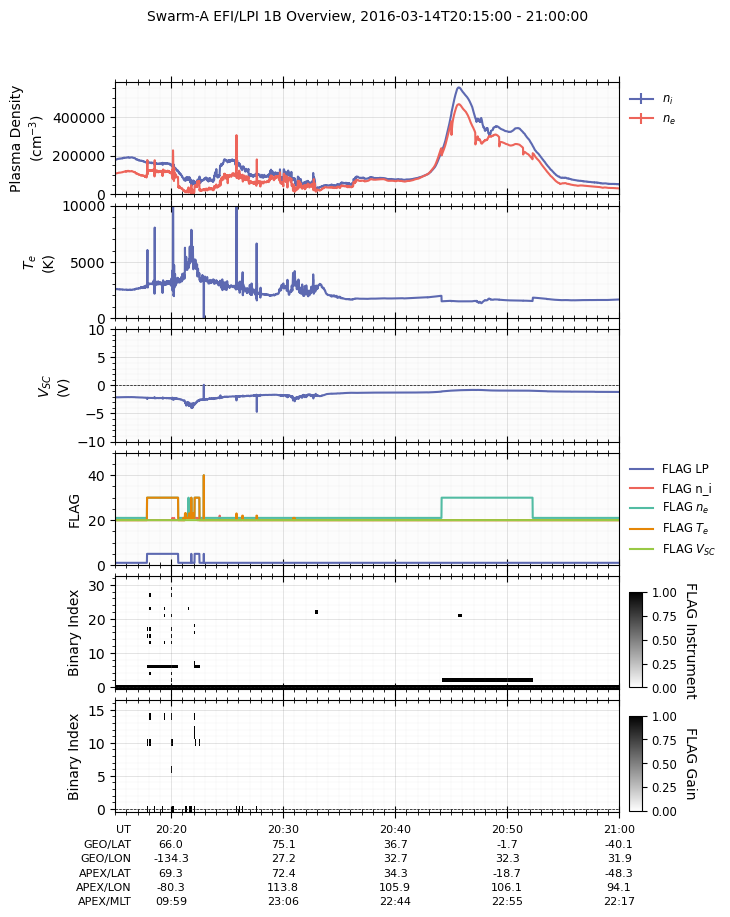
\includegraphics[width=0.7\linewidth]{files/834e3e20a3083951b5b314c059207316.png}

\paragraph{Swarm EFI LP FP data}

\begin{verbatim}
def test_swarm_EFI_LP_FP_overview():
    """Test Swarm EFI/LP -FP data product
    
    """
    dt_fr = datetime.datetime(2016, 3, 14, 20, 15)
    dt_to = datetime.datetime(2016, 3, 14, 21, 0)

    db = dashboards.TSDashboard(
        dt_fr=dt_fr, dt_to=dt_to, figure_config={'figsize': (8, 10)},
        timeline_extra_labels=['GEO_LAT', 'GEO_LON', 'APEX_LAT', 'APEX_LON', 'APEX_MLT'],
        )

    ds = db.dock(
        datasource_contents=['esa_eo', 'swarm', 'advanced', 'efi_lp_fp'], 
        product_version='latest', # 'latest' (default),
        sat_id='A', add_APEX=True)
    
    panel_layouts = [
        [ds['n_p']],
        [ds['I_FP']],
    ]
    
    db.set_layout(panel_layouts=panel_layouts)
    db.draw()
    db.add_title(title='Swarm -{} EFI/LP -FP Overview'.format(ds.sat_id), fontsize='medium', append_time=True)

    db.show()
test_swarm_EFI_LP_FP_overview()
\end{verbatim}

\begin{verbatim}
Create a new figure: Figure(800x1000).
Searching the data product "EFI_LP_FP" with the version "latest" on the server...
The file [PosixPath('/data/afys -ionosphere/data/ESA/SWARM/Advanced/EFI_LP_FP/0203/Sat_A/2016/SW_EXTD_EFIA_LP_FP_20160314T063806_20160314T235959_0203.cdf')] already exists: skip downloading.
\end{verbatim}

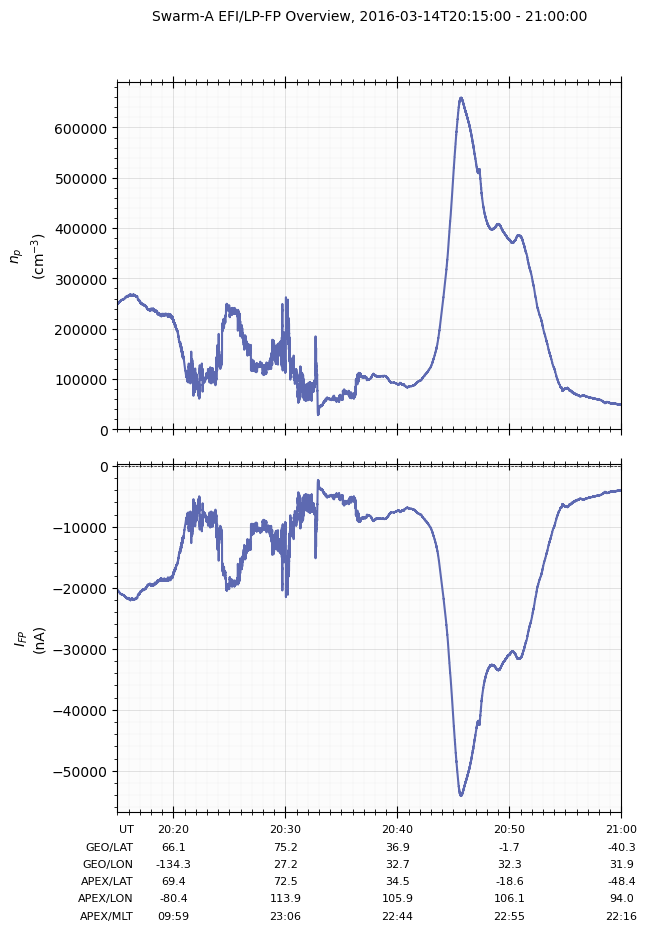
\includegraphics[width=0.7\linewidth]{files/fe18e90b6d1237b3afdce05e2aa707ae.png}

\paragraph{Swarm EFI LP HM data}

\begin{verbatim}
def test_swarm_EFI_LP_HM_overview():
    """Test Swarm EFI/LP -HM data product
    
    """
    dt_fr = datetime.datetime(2016, 3, 14, 20, 15)
    dt_to = datetime.datetime(2016, 3, 14, 21, 0)

    db = dashboards.TSDashboard(
        dt_fr=dt_fr, dt_to=dt_to, figure_config={'figsize': (8, 10)},
        timeline_extra_labels=['GEO_LAT', 'GEO_LON', 'APEX_LAT', 'APEX_LON', 'APEX_MLT'],
        )

    ds = db.dock(
        datasource_contents=['esa_eo', 'swarm', 'advanced', 'efi_lp_hm'], 
        product_version='latest', # 'latest' (default),
        sat_id='A', add_APEX=True)
    
    panel_layouts = [
        [ds['n_p']],
        [ds['T_e'], ds['T_e_HG'], ds['T_e_LG']],
        [ds['V_SC_HG'], ds['V_SC_LG']],
        [ds['FLAG_BIN_AUX'],],
    ]
    
    ds['T_e'].visual.axis[1].lim = [ -10, 10000]
    
    db.set_layout(panel_layouts=panel_layouts)
    db.draw()
    db.add_title(title='Swarm -{} EFI/LP -HM Overview'.format(ds.sat_id), fontsize='medium', append_time=True)

    db.show()
test_swarm_EFI_LP_HM_overview()
\end{verbatim}

\begin{verbatim}
Create a new figure: Figure(800x1000).
Searching the data product "EFI_LP_HM" with the version "latest" on the server...
The file [PosixPath('/data/afys -ionosphere/data/ESA/SWARM/Advanced/EFI_LP_HM/0102/Sat_A/2016/SW_EXTD_EFIA_LP_HM_20160314T000000_20160314T235959_0102.cdf')] already exists: skip downloading.
\end{verbatim}

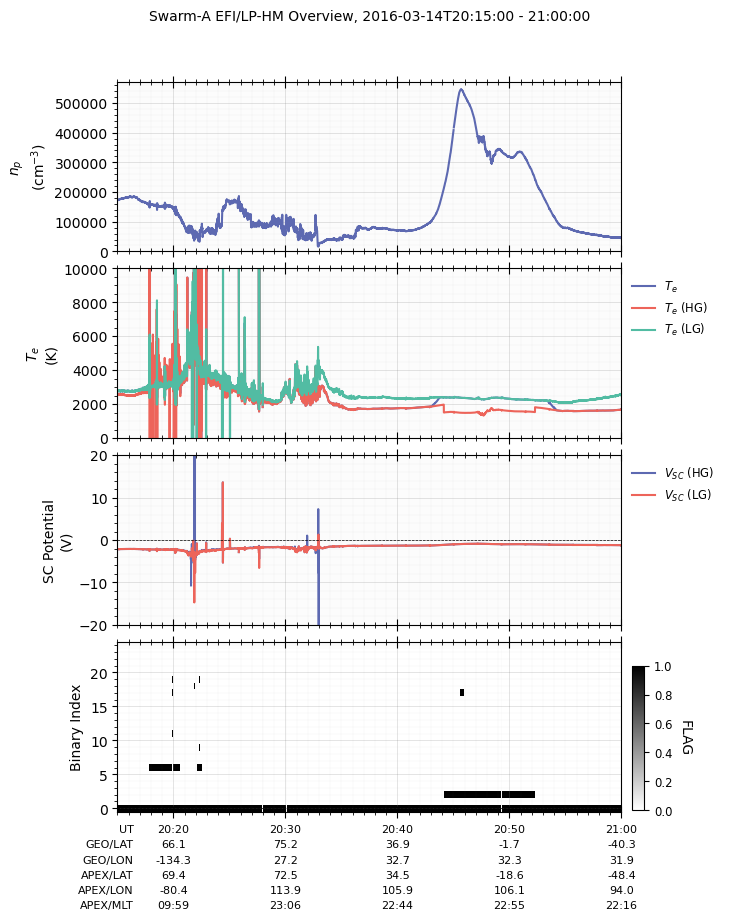
\includegraphics[width=0.7\linewidth]{files/f587d7fbc3a83824115bd14d99fb3623.png}

\paragraph{A combination of different EFI data products}

\begin{verbatim}
def test_swarm_compare_EFI_LP_FP_HM():
    """Test Swarm EFI/LP -FP vs. EFI/LP -HM data products
    
    """
    dt_fr = datetime.datetime(2016, 3, 14, 20, 15)
    dt_to = datetime.datetime(2016, 3, 14, 20, 35)

    db = dashboards.TSDashboard(
        dt_fr=dt_fr, dt_to=dt_to, figure_config={'figsize': (8, 10)},
        timeline_extra_labels=['GEO_LAT', 'GEO_LON', 'APEX_LAT', 'APEX_LON', 'APEX_MLT'],
        )

    ds_lp_fp = db.dock(
        datasource_contents=['esa_eo', 'swarm', 'advanced', 'efi_lp_fp'], 
        product_version='latest', # 'latest' (default),
        sat_id='A', add_APEX=True)
    
    ds_lp_1b = db.dock(
        datasource_contents=['esa_eo', 'swarm', 'l1b', 'efi_lp'], 
        product_version='latest', # 'latest' (default),
        sat_id='A', add_APEX=True)
    
    ds_lp_hm = db.dock(
        datasource_contents=['esa_eo', 'swarm', 'advanced', 'efi_lp_hm'], 
        product_version='latest', # 'latest' (default),
        sat_id='A', add_APEX=True)
    
    panel_layouts = [
        [ds_lp_fp['n_p'], ds_lp_1b['n_i'], ds_lp_1b['n_e'], ds_lp_hm['n_p']],
        [ds_lp_1b['T_e'], ds_lp_hm['T_e'], ds_lp_hm['T_e_HG'], ds_lp_hm['T_e_LG']],
        [ds_lp_1b['FLAG_LP'], ds_lp_1b['FLAG_n_i'], ds_lp_1b['FLAG_n_e'], ds_lp_1b['FLAG_T_e'], ds_lp_1b['FLAG_V_SC']],
        [ds_lp_1b['FLAG_1_BIN_AUX'],],
        [ds_lp_1b['FLAG_2_BIN_AUX'],],
        [ds_lp_hm['FLAG_BIN_AUX'],],
    ]
    ds_lp_1b['n_i'].visual.axis[2].label = r"n$_i$ (1B)"
    ds_lp_1b['n_e'].visual.axis[2].label = r"n$_e$ (1B)"
    ds_lp_1b['T_e'].visual.axis[2].label = r"T$_e$ (1B)"
    ds_lp_fp['n_p'].visual.axis[2].label = r"n$_p$ (FP)"
    ds_lp_hm['n_p'].visual.axis[2].label = r"n$_p$ (HM)"
    ds_lp_hm['T_e'].visual.axis[2].label = r"T$_e$ (HM)"
    ds_lp_hm['T_e_HG'].visual.axis[2].label = r"T$_e$ (HG)"
    ds_lp_hm['T_e_LG'].visual.axis[2].label = r"T$_e$ (LG)"
    ds_lp_1b['T_e'].visual.axis[1].lim = [ -10, 10000]
    
    db.set_layout(panel_layouts=panel_layouts)
    db.draw()
    db.add_title(title='Swarm -{} EFI/LP 1B vs FP vs HM Comparison'.format(ds_lp_fp.sat_id), fontsize='medium', append_time=True)

    db.show()
test_swarm_compare_EFI_LP_FP_HM()
\end{verbatim}

\begin{verbatim}
Create a new figure: Figure(800x1000).
Searching the data product "EFI_LP_FP" with the version "latest" on the server...
The file [PosixPath('/data/afys -ionosphere/data/ESA/SWARM/Advanced/EFI_LP_FP/0203/Sat_A/2016/SW_EXTD_EFIA_LP_FP_20160314T063806_20160314T235959_0203.cdf')] already exists: skip downloading.
Searching the data product "EFI_LP" with the version "latest" on the server...
The file [PosixPath('/data/afys -ionosphere/data/ESA/SWARM/Level1b/EFI_LP/0701/Sat_A/2016/SW_OPER_EFIA_LP_1B_20160314T000000_20160314T235959_0701_MDR_EFI_LP.cdf')] already exists: skip downloading.
Searching the data product "EFI_LP_HM" with the version "latest" on the server...
The file [PosixPath('/data/afys -ionosphere/data/ESA/SWARM/Advanced/EFI_LP_HM/0102/Sat_A/2016/SW_EXTD_EFIA_LP_HM_20160314T000000_20160314T235959_0102.cdf')] already exists: skip downloading.
\end{verbatim}

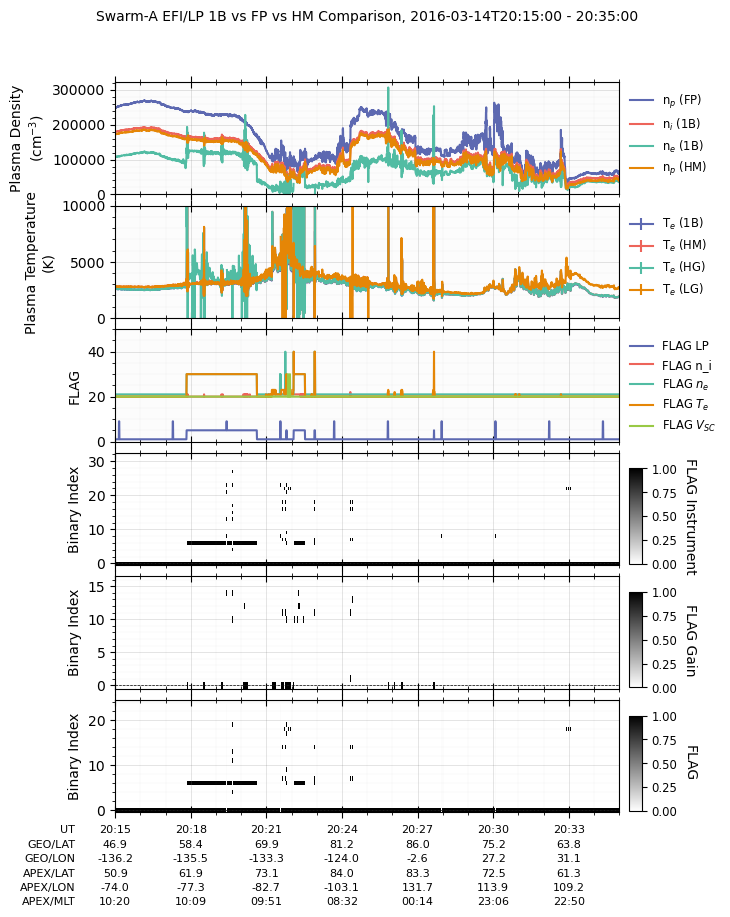
\includegraphics[width=0.7\linewidth]{files/0414ee2df957691c9b6bdbb1e8c5dd9b.png}